\subsection{Measured Differential Cross-sections}
\label{diff-xs}

Differential cross-sections are measured in the fiducial phase spaces by counting data events in each bin of the relevant observables, subtracting the expected background contributions, and correcting for detector effects. Detector-level distributions are unfolded to stable-particle level using an iterative Bayesian method~\cite{DAgostini1995}, which accounts for resolution effects, reconstruction inefficiencies, and bin migrations. Response matrices derived from simulated signal samples encode the probability of an event generated in a given particle-level bin being reconstructed in a corresponding detector-level bin. 

The number of iterations, typically between two and five depending on the observable, is optimised to balance statistical uncertainty and unfolding stability. The binning is defined using purity and efficiency criteria to ensure reliable unfolding and preserve the distribution shapes. The final bin of each observable is open-ended and extends to the kinematic limit, with no separate overflow bin. Validation studies using nominal and alternative samples show no significant bias. 
The kinematic variables used for the differential cross-section measurements are summarised in Table~\ref{tab:diff-var}.
\begin{table}[!hbtp]
    \centering
    \scriptsize
    \renewcommand{\arraystretch}{1.5}
    \begin{tabular}{l c c}
    \hline
  \textbf{Observable description} &  \textbf{Observable} &  \textbf{SR} \\
     \hline 
      Azimuthal angular separation of the two leptons & $\Delta\phi(\ell, \ell)$  & $ZZ$ and $ZZjj$ \\
      Transverse momentum of the leading lepton  &  $p_\text{T}^{\text{leading lepton}}$ & $ZZ$ only \\  
      Transverse momentum of the Z boson  & $p_\text{T}^Z$ & $ZZ$ and $ZZjj$ \\  
      Rapidity of the visible $Z \rightarrow \ell\ell$  &    $|y^Z|$ & $ZZ$ and $ZZjj$ \\ 
      Transverse momentum of the $ZZ$ system  &  $p_\text{T}^{ZZ}$ & $ZZ$ and $ZZjj$ \\ 
       Transverse mass of the $ZZ$ system 
       &  $m_\text{T}^{ZZ}$ & $ZZ$ and $ZZjj$\\
     Number of jets                   &   $N_{jets}$ & $ZZ$ only\\  
 %   CP-sensitive angular variable (scenario 1)  & $sin(\phi_1)cos(\theta_1)$ & $ZZ$ only \\  \hline 
    CP-sensitive angular variable   &  $\sin(\varphi)\cos(\theta)$ & $ZZ$ only\\
    Invariant mass of the dijet system & $m_{jj}$ & $ZZjj$ only \\ 
    Transverse momentum of the leading jet & $p_\text{T}^{\text{leading jet}}$ & $ZZjj$ only \\ 
    \hline
    \end{tabular}
    \caption{\rm Kinematic variables for the differential cross-section measurements.} %through the unfolding procedure.}
    \label{tab:diff-var}
\end{table} 

A CP-sensitive angular variable, $\sin\varphi \cos\theta$, is constructed in the $ZZ$ signal region following Refs.~\cite{Chang:1994cs, STDM-2021-05, Semushin:2025uts}. The polar angle $\theta$ and azimuthal angle $\varphi$ are defined for the negatively charged lepton in the dilepton rest frame, with the $z$-axis aligned with the dilepton momentum in the $ZZ$ rest frame and the remaining axes forming a right-handed coordinate system. Since neutrinos from $Z\to\nu\bar{\nu}$ decays are not directly detected, the dineutrino momentum is approximated as $\vec{p}^{\,\nu\nu}=-\vec{p}^{\,\ell\ell}$, corresponding to the assumption that the $ZZ$ system is at rest in the laboratory frame. The differential cross-section for this observable is unfolded to particle level in the fiducial phase space.

Figures~\ref{fig:diff-xs-ZZ} and~\ref{fig:diff-xs-ZZjj} present the measured differential cross-sections. The quoted uncertainties include both statistical and systematic contributions propagated through the unfolding procedure. Statistical uncertainties dominate most bins, while systematic uncertainties become significant in specific kinematic regions.

The measured differential cross-sections in the $ZZ$ fiducial phase space show good agreement with SM predictions from the nominal \textsc{Sherpa}+\textsc{MadGraph5} simulation (denoted as \textsc{Sherpa+MG5}) and from the \textsc{Matrix} calculation. The \textsc{Matrix} predictions show slightly improved agreement with the data, consistent with the inclusion of NNLO QCD corrections.

In the $ZZjj$ fiducial phase space, the results are compared with SM predictions obtained using \textsc{Sherpa} for strong production and \textsc{MadGraph5} for electroweak production. The total uncertainties in the $ZZjj$ measurements are larger than those in the inclusive $ZZ$ phase space due to reduced event statistics and additional jet-related uncertainties. The \textsc{Sherpa} prediction describes the data well within uncertainties.


%%% differential cross-section Plots
\begin{figure}[!hbtp]
    \centering
    \subfloat[]{
    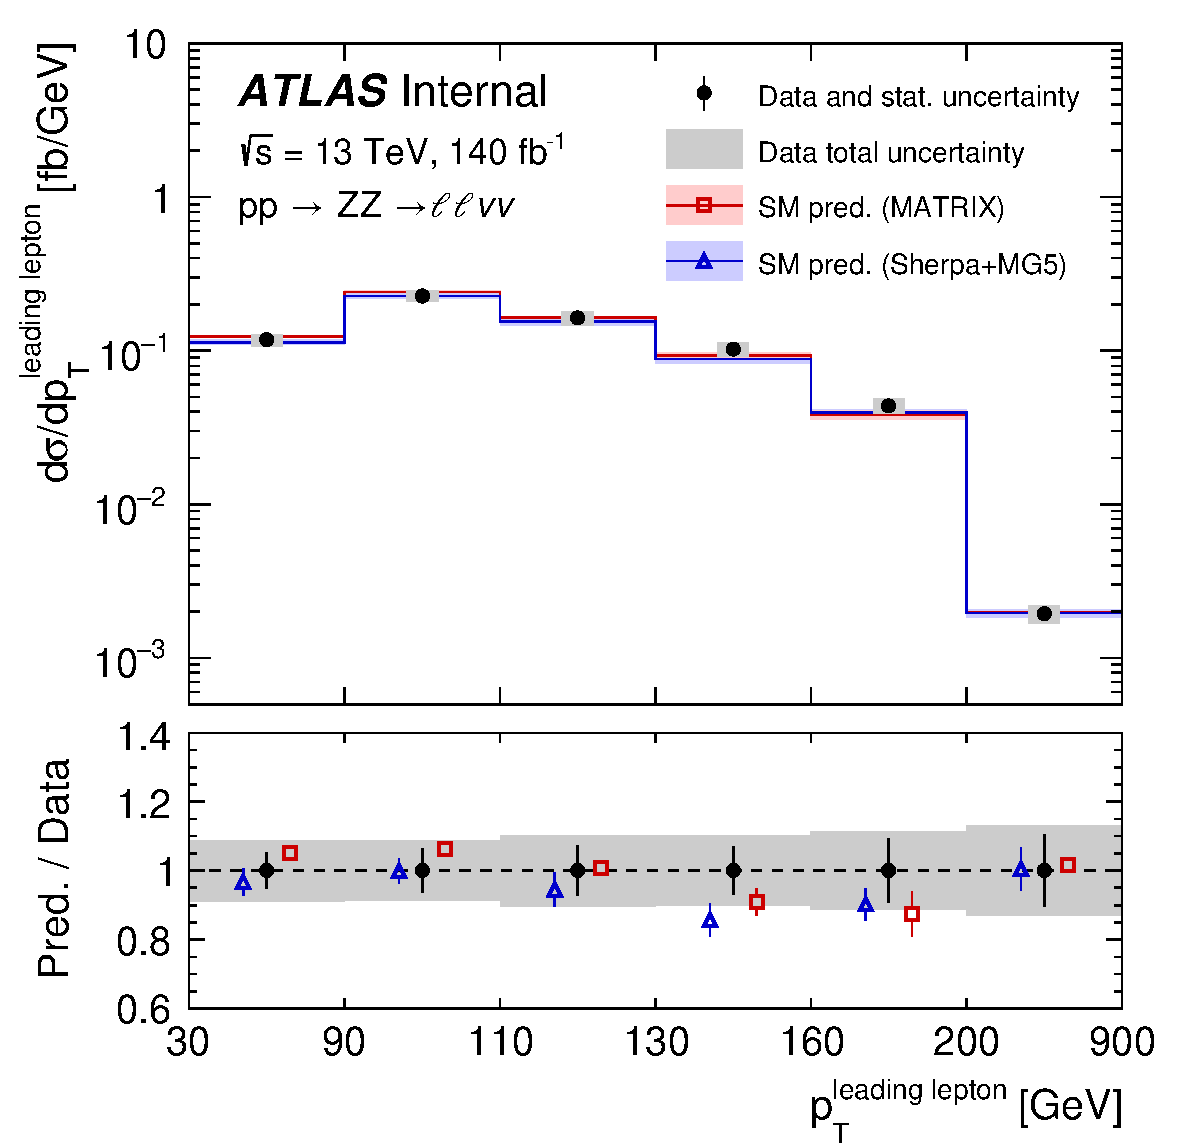
\includegraphics[width=0.32\linewidth]{figures/ch5-llvv/diff-xs/ZZ-pT_l1.pdf}
    }
    \subfloat[]{
    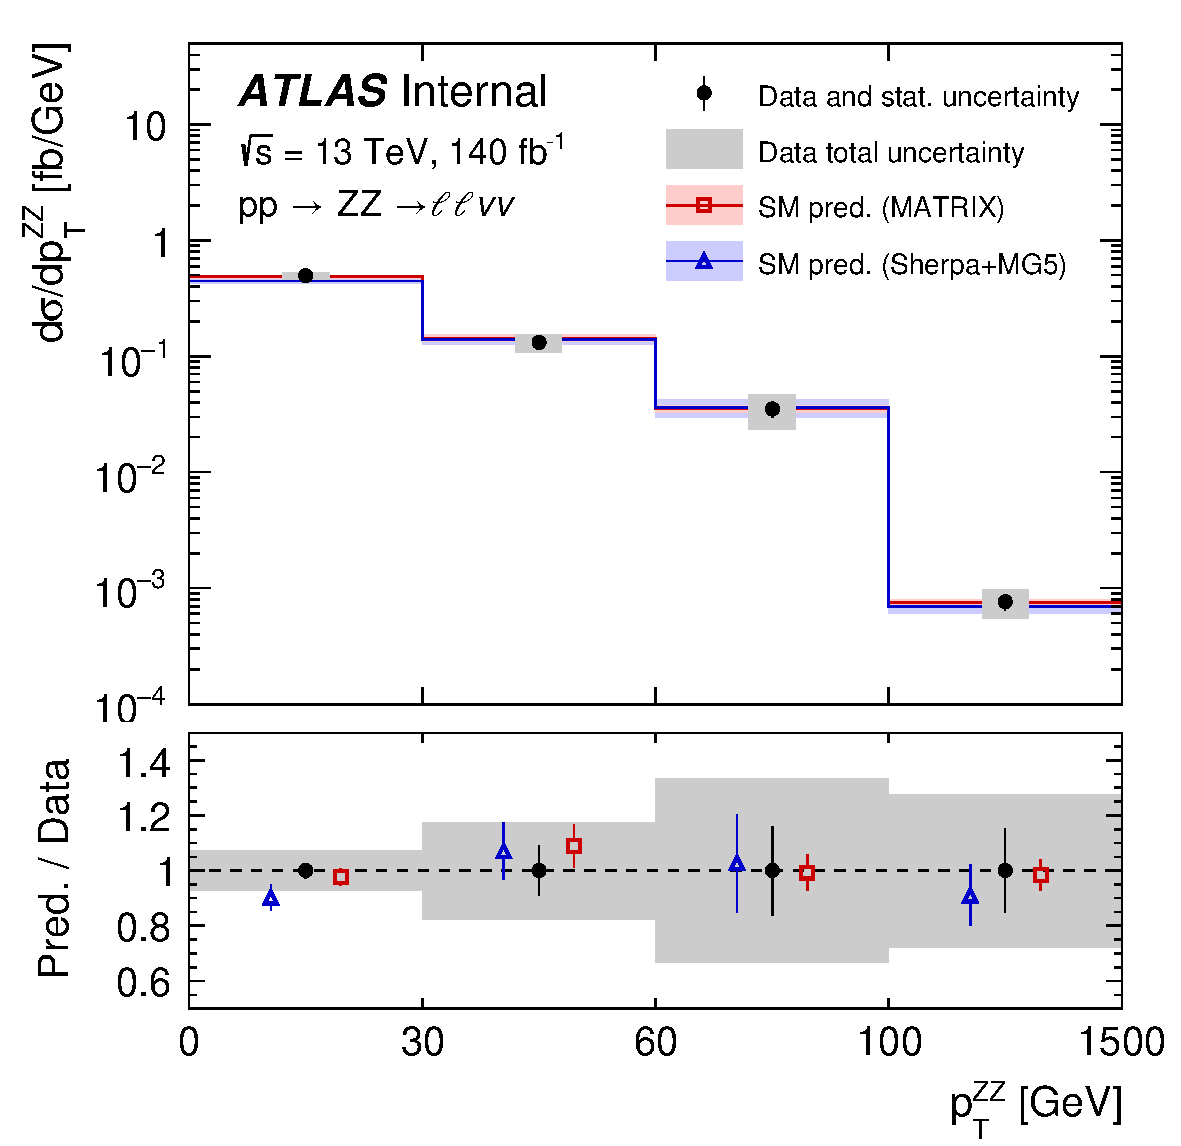
\includegraphics[width=0.32\linewidth]{figures/ch5-llvv/diff-xs/ZZ-pT_ZZ.pdf}
    }
    \subfloat[]{    
    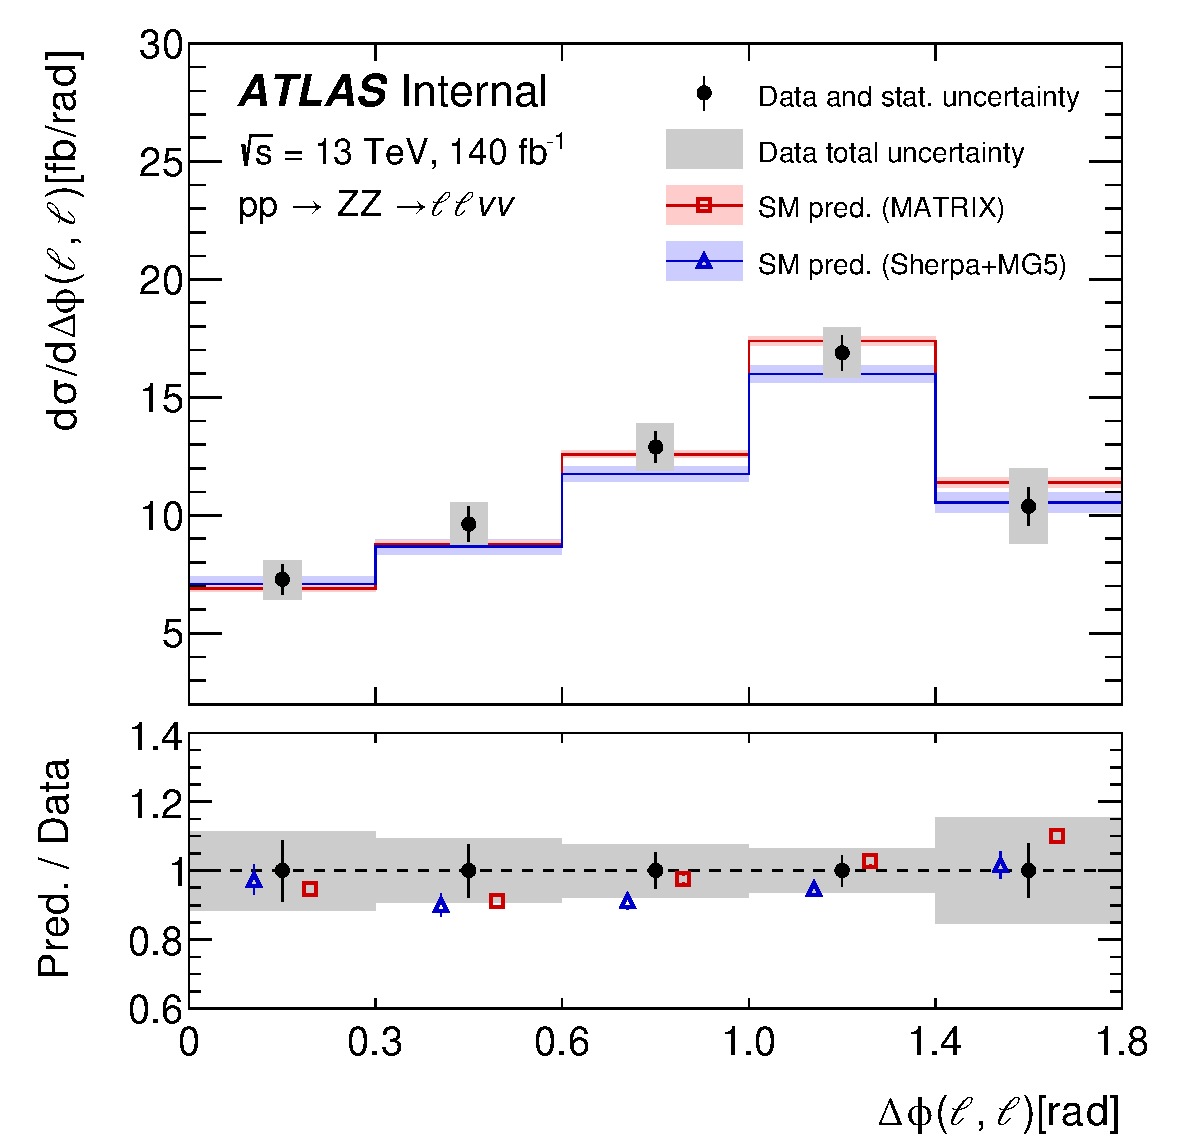
\includegraphics[width=0.32\linewidth]{figures/ch5-llvv/diff-xs/ZZ-dphi_ll.pdf}
    }\\
    \subfloat[]{    
    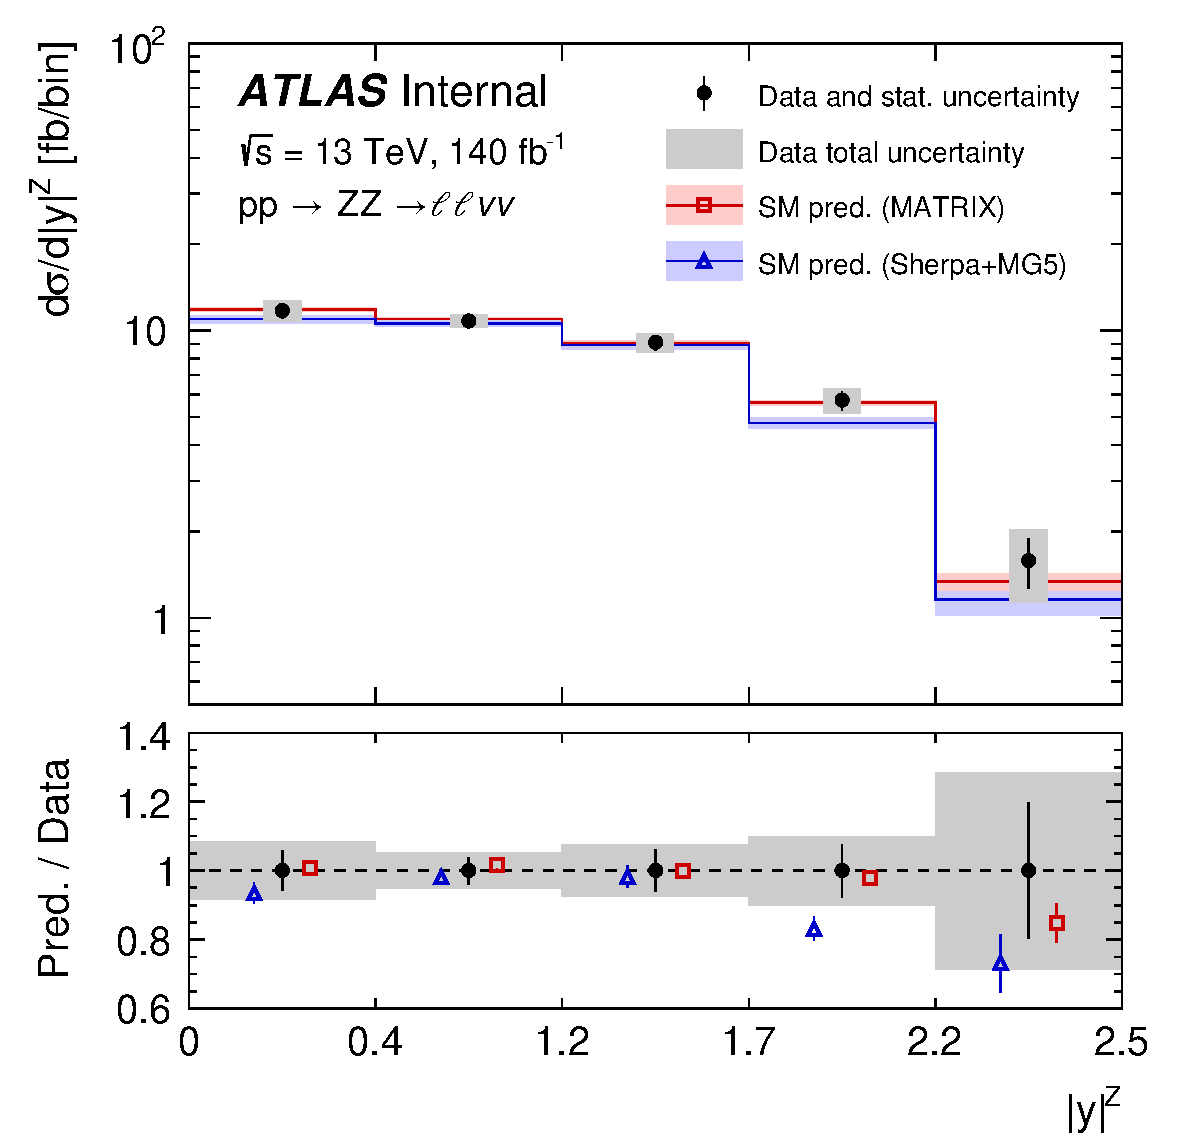
\includegraphics[width=0.32\linewidth]{figures/ch5-llvv/diff-xs/ZZ-y_Z.pdf}
    }
    \subfloat[]{    
    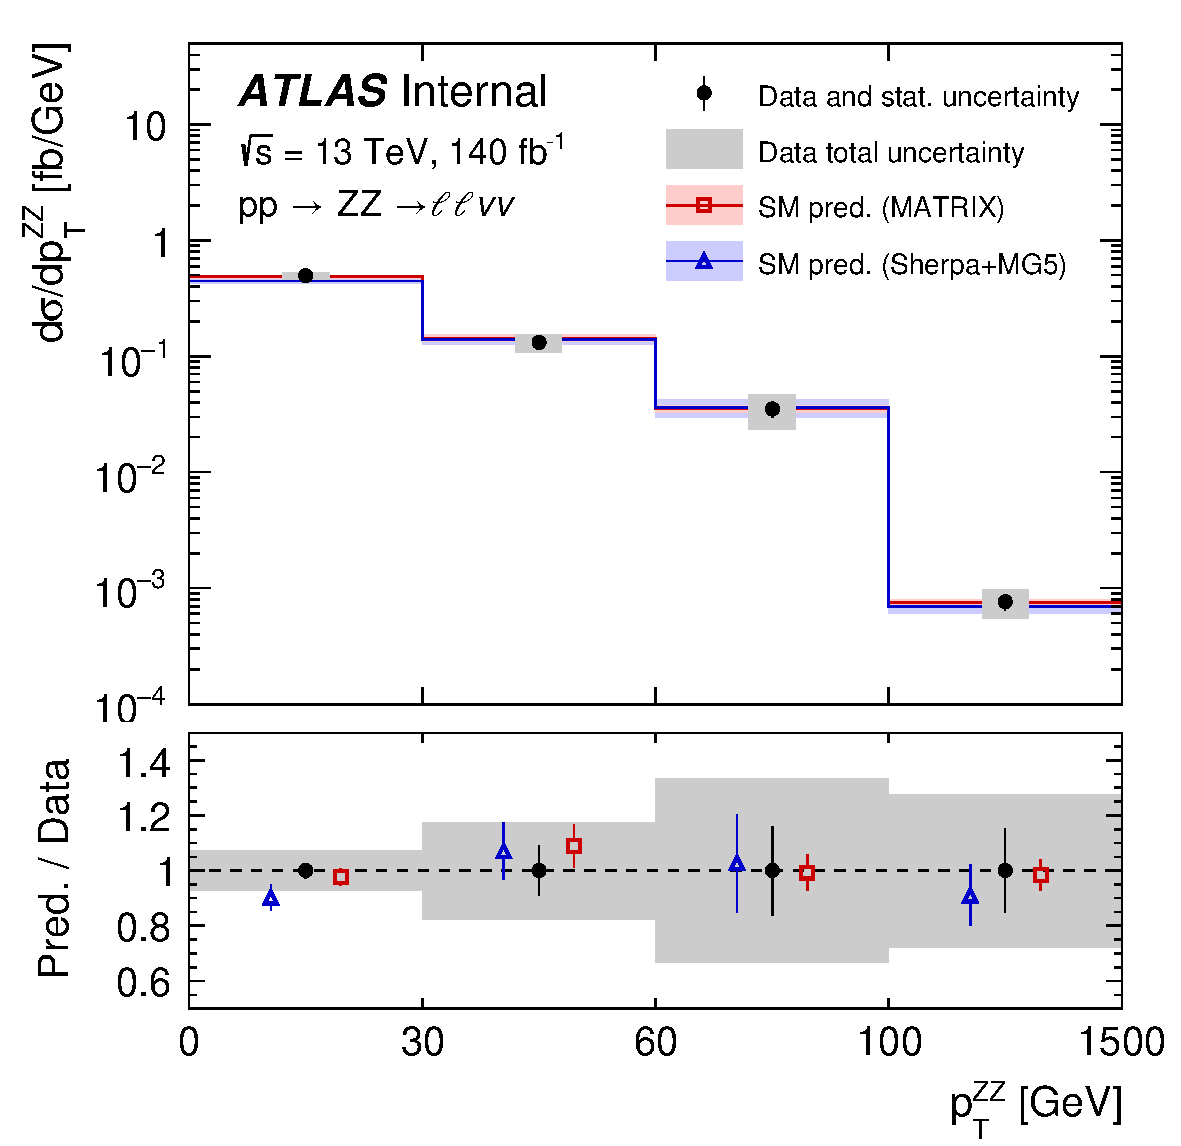
\includegraphics[width=0.32\linewidth]{figures/ch5-llvv/diff-xs/ZZ-pT_ZZ.pdf}
    }
    \subfloat[]{    
    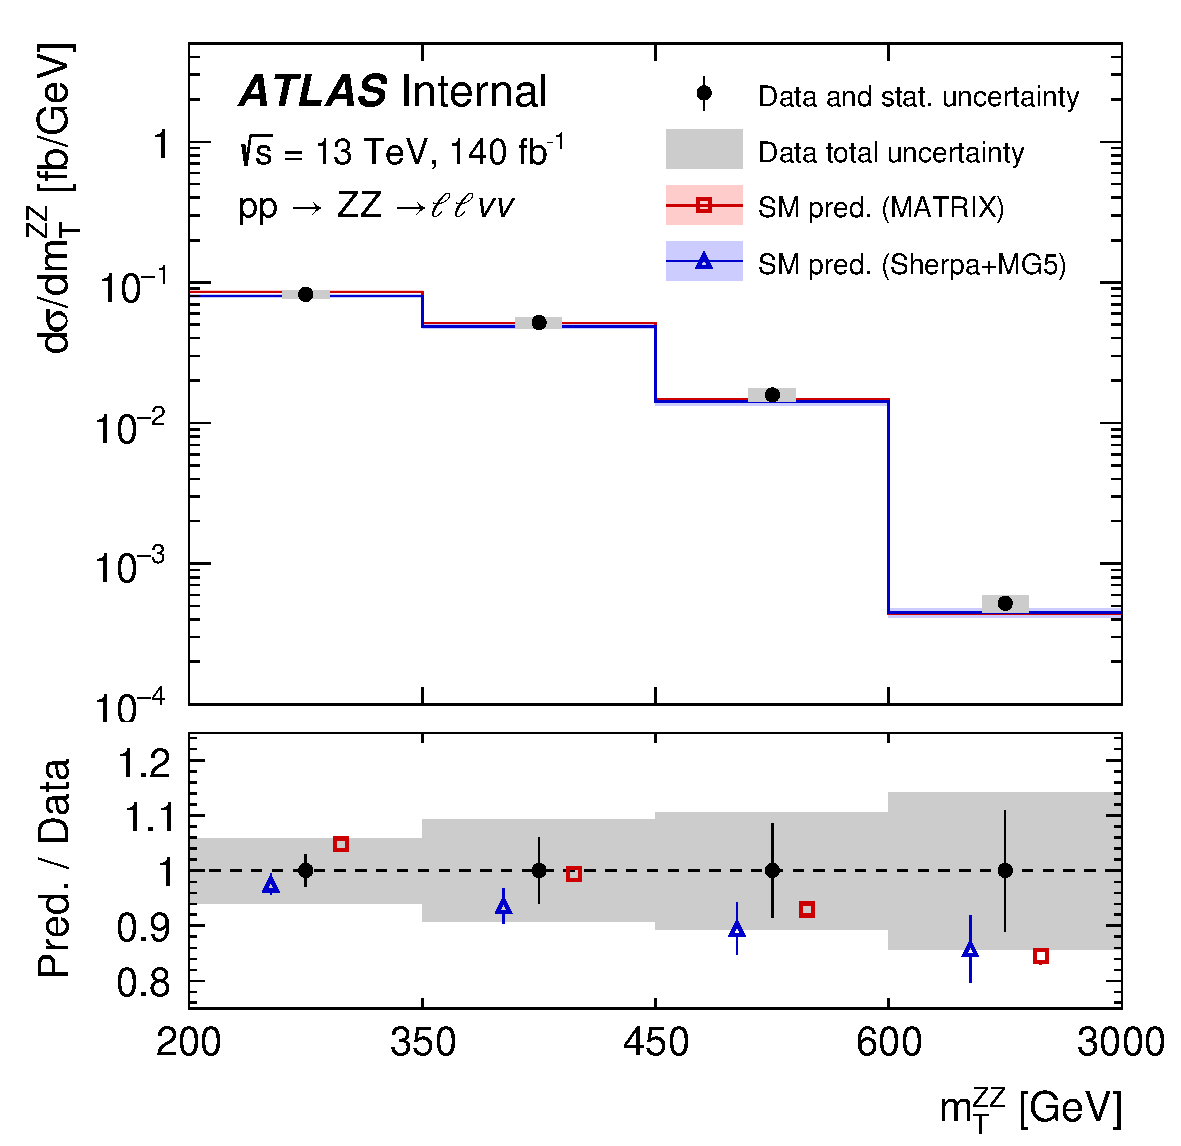
\includegraphics[width=0.32\linewidth]{figures/ch5-llvv/diff-xs/ZZ-mT_ZZ.pdf}
    }\\
    \subfloat[]{    
    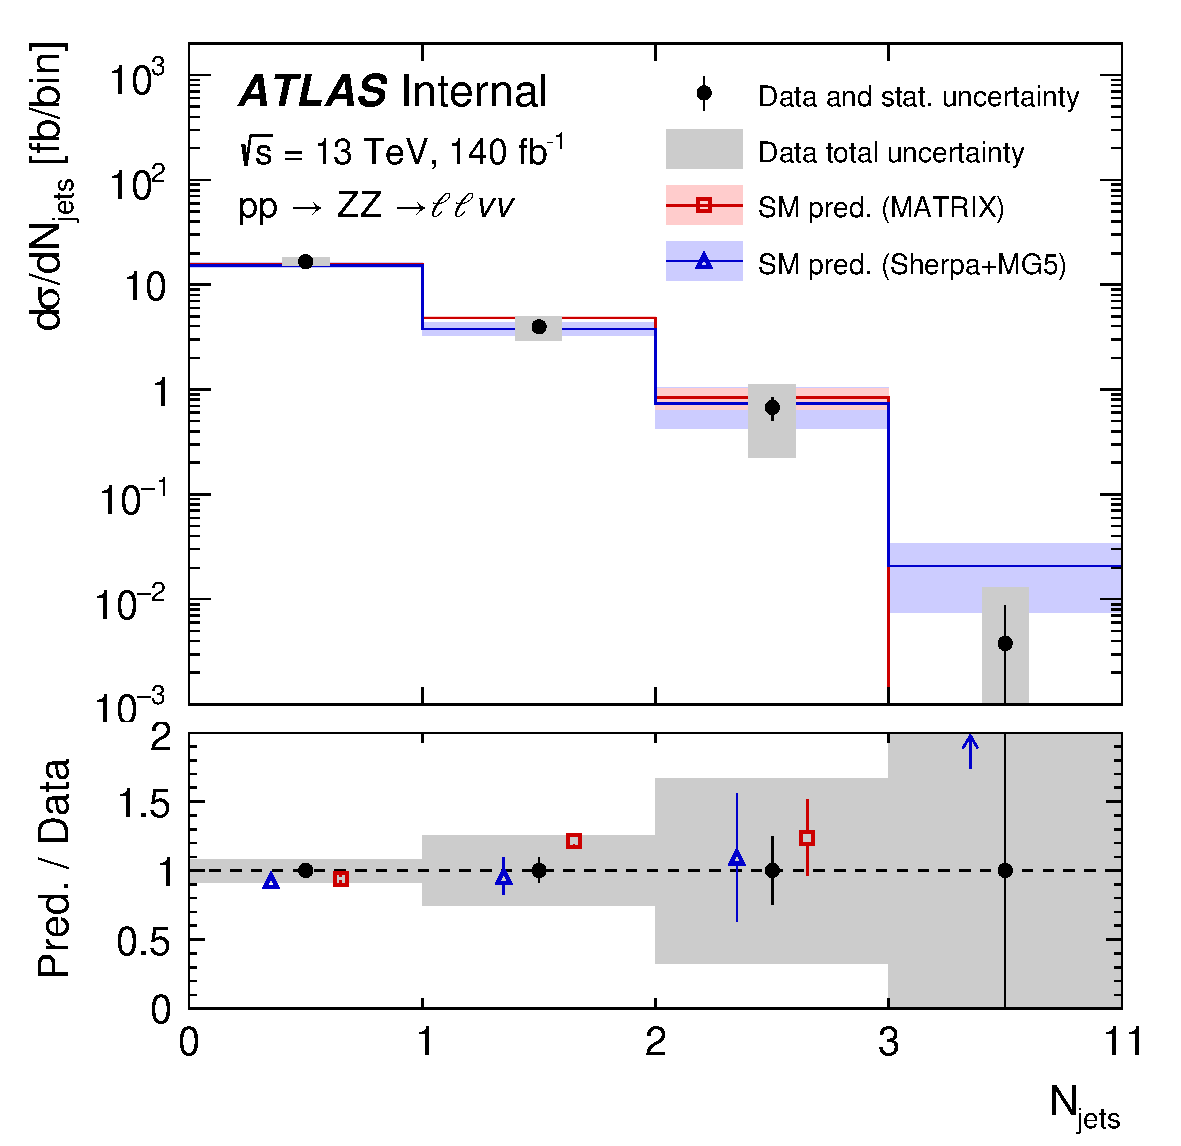
\includegraphics[width=0.32\linewidth]{figures/ch5-llvv/diff-xs/ZZ-njets.pdf} 
    }
    \subfloat[]{    
    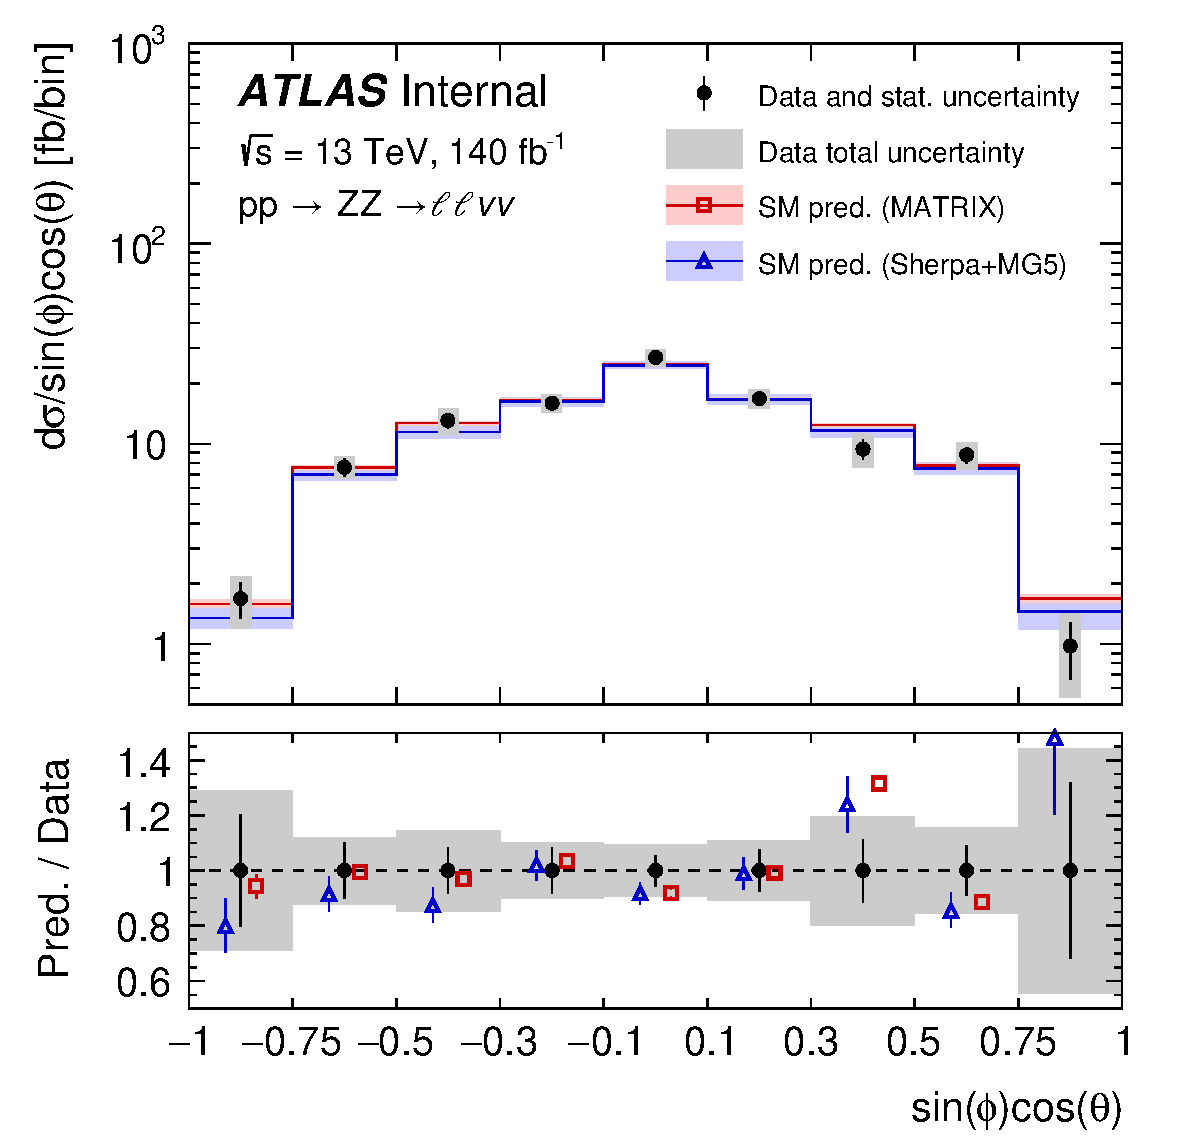
\includegraphics[width=0.32\linewidth]{figures/ch5-llvv/diff-xs/ZZ-sincos_2.pdf}
    }
    \caption{Differential cross-section measurements in the inclusive $ZZ\rightarrow \ell\ell\nu\nu$ fiducial phase space, compared with MC predictions calculated by the nominal \textsc{Sherpa} simulation %(denoted as \textsc{Sherpa})
    and by \textsc{Matrix} for a set of kinematic variables:
(a) $p_\text{T}^\text{leading lepton}~,
\text{(b)}~ p_\text{T}^\text{Z}~,
\text{(c)}~\Delta\phi(\ell, \ell),~
\text{(d)}~|y^Z|,~
\text{(e)}~ p_\text{T}^\text{ZZ},~
\text{(f)}~ m_\text{T}^\text{ZZ},~
\text{(g)}~ N_\text{jets}$,
and (h) a CP-sensitive angular variable, $\sin(\varphi)\cos(\theta)$.
The statistical and total uncertainties on the data points are displayed in both the differential cross-sections and the corresponding ratios. The total theoretical uncertainties for the \textsc{Sherpa} and \textsc{Matrix} predictions are represented as shaded bands in the cross-section panels and as error bars in the ratio panels.
}
\label{fig:diff-xs-ZZ}
\end{figure}


\begin{figure}[!hbtp]
    \centering
    \subfloat[]{  
    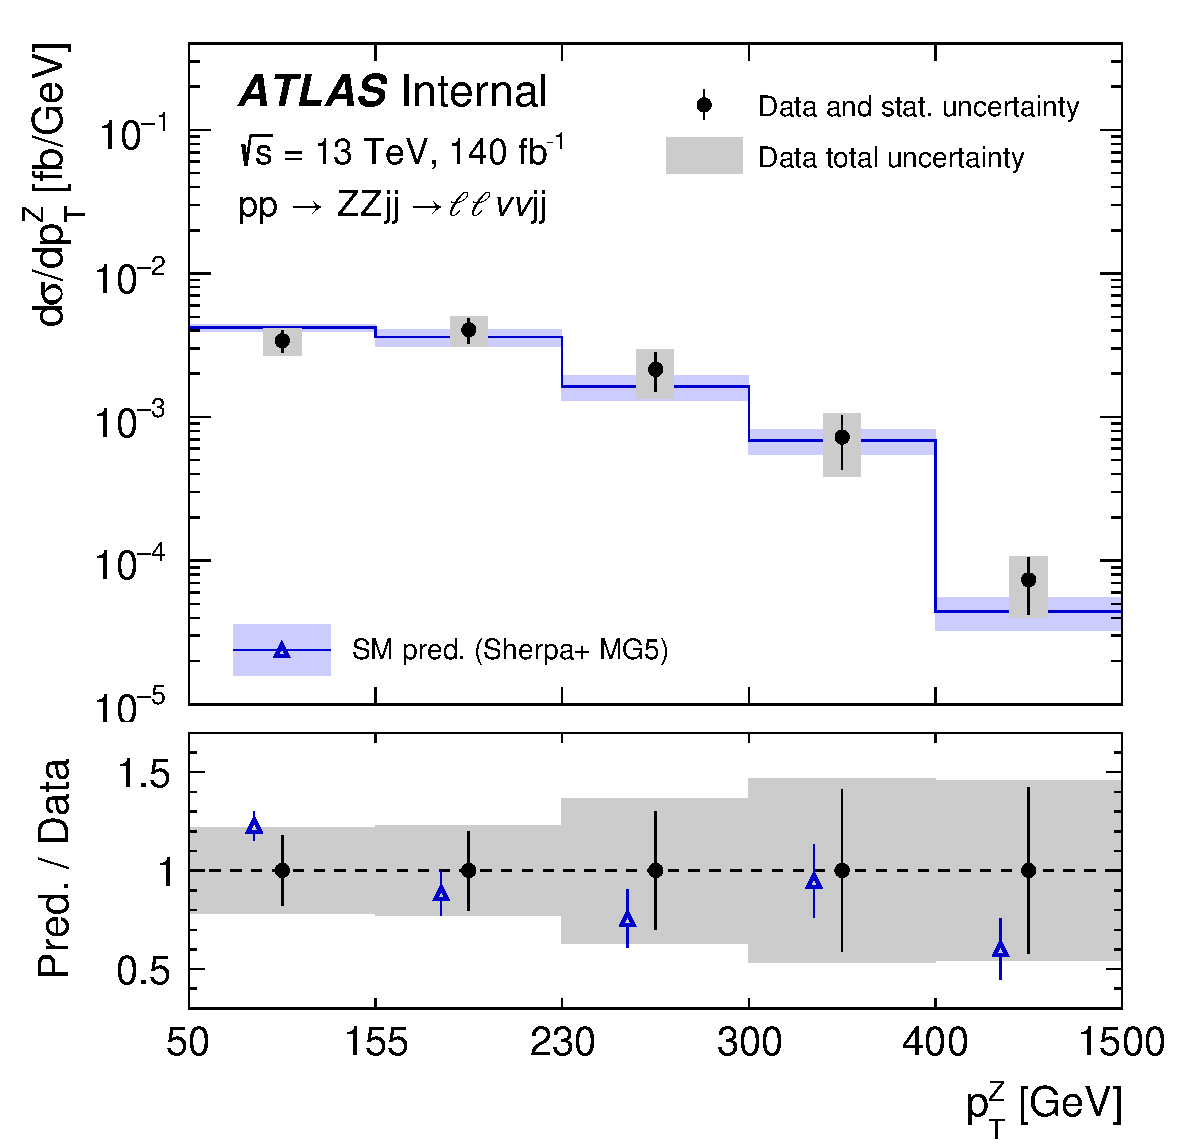
\includegraphics[width=0.32\linewidth]{figures/ch5-llvv/diff-xs/ZZjj-pT-Z.pdf}
    }
    \subfloat[]{  
    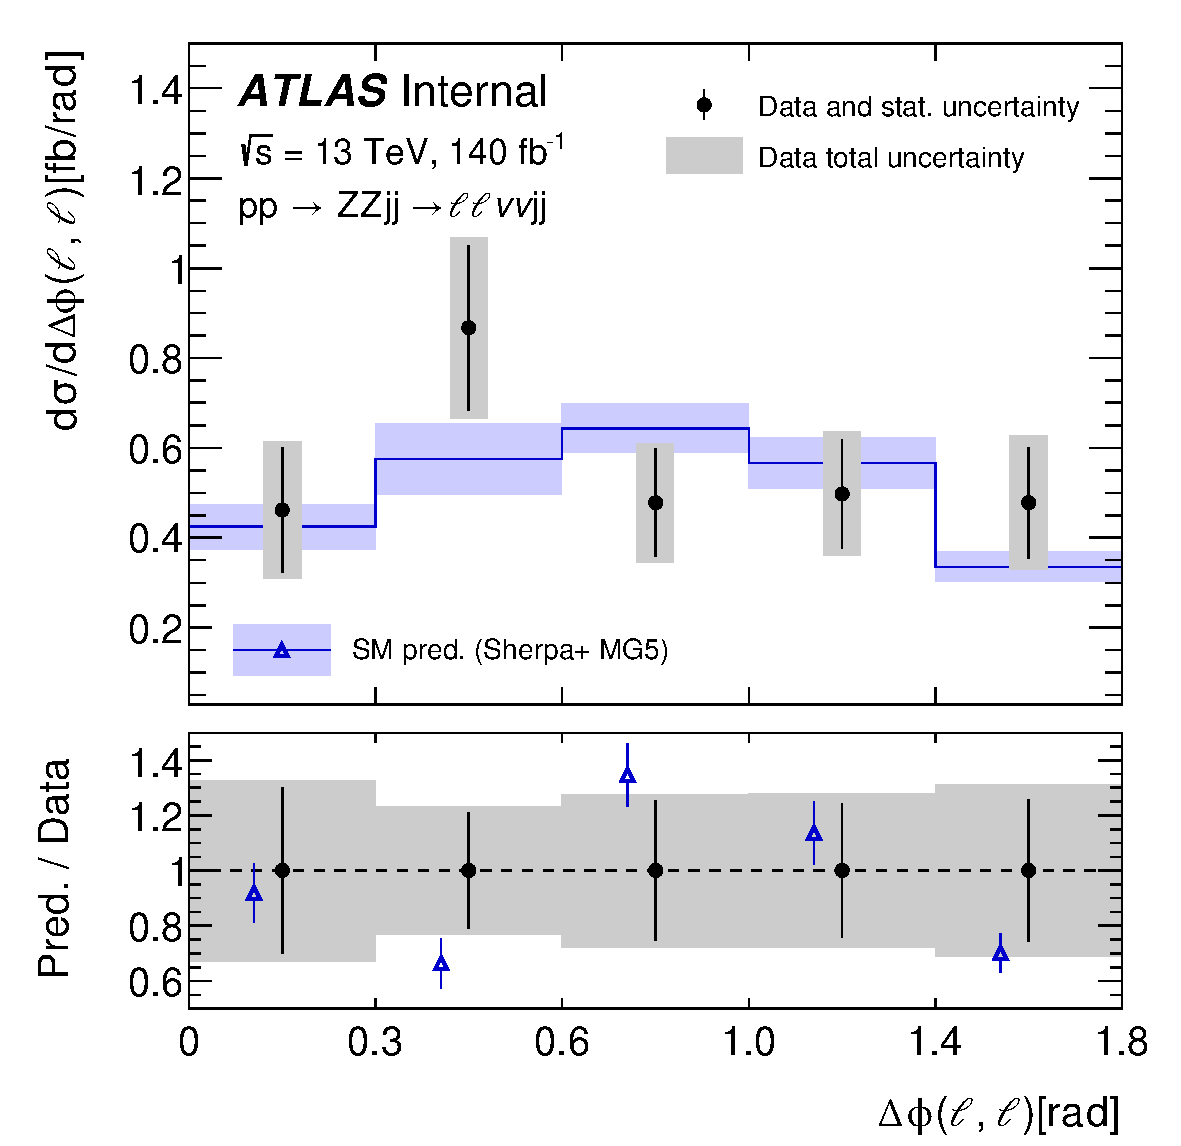
\includegraphics[width=0.32\linewidth]{figures/ch5-llvv/diff-xs/ZZjj-Dphi-ll.pdf}
    }
    \subfloat[]{  
    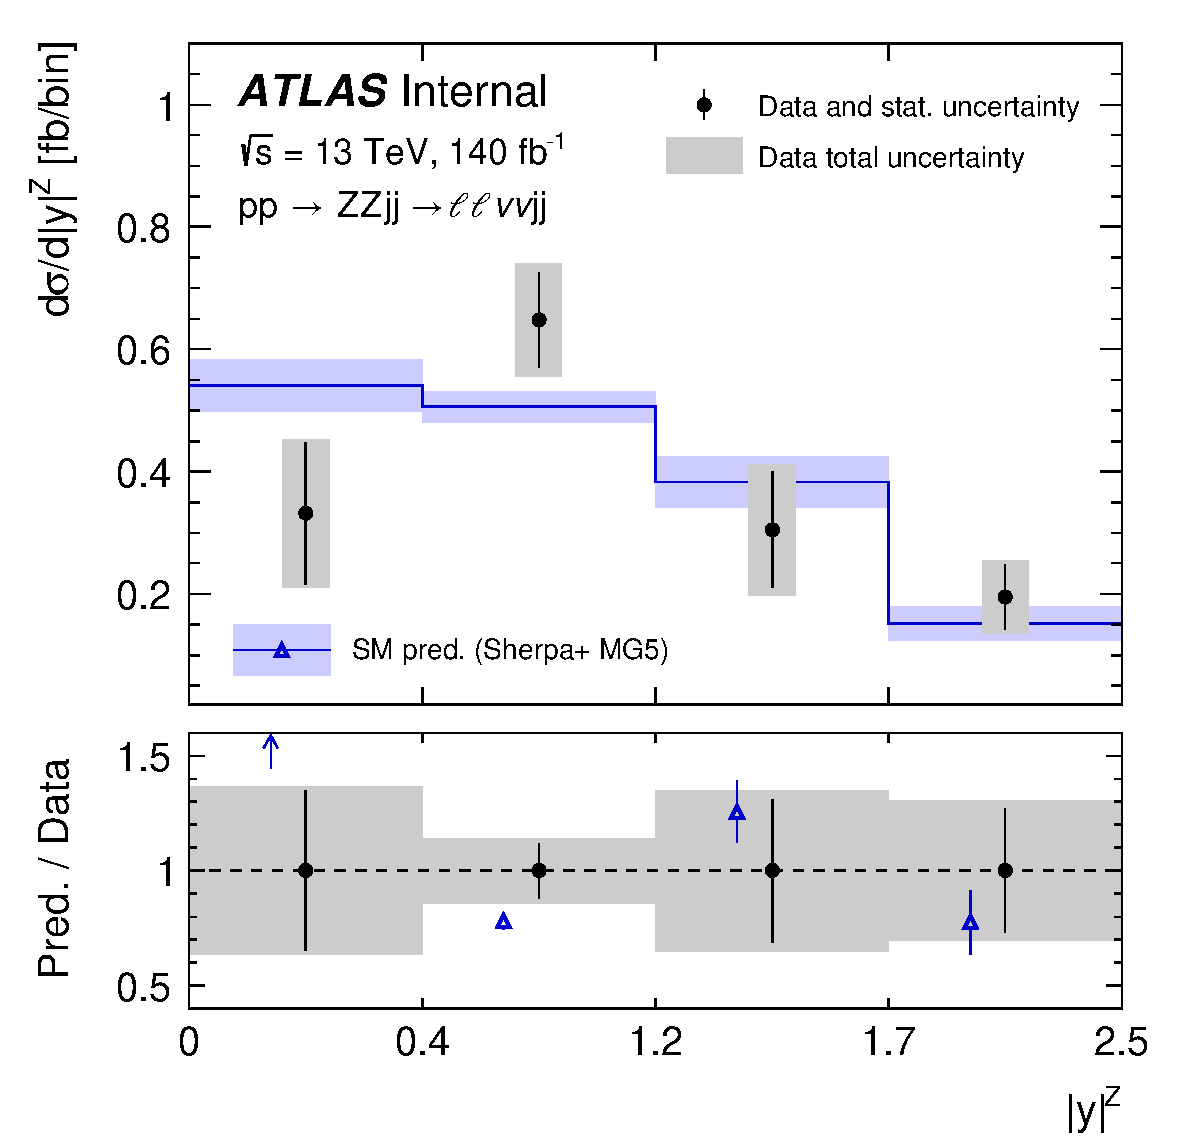
\includegraphics[width=0.32\linewidth]{figures/ch5-llvv/diff-xs/ZZjj-Y-Z.pdf}
    }\\
    \subfloat[]{      
    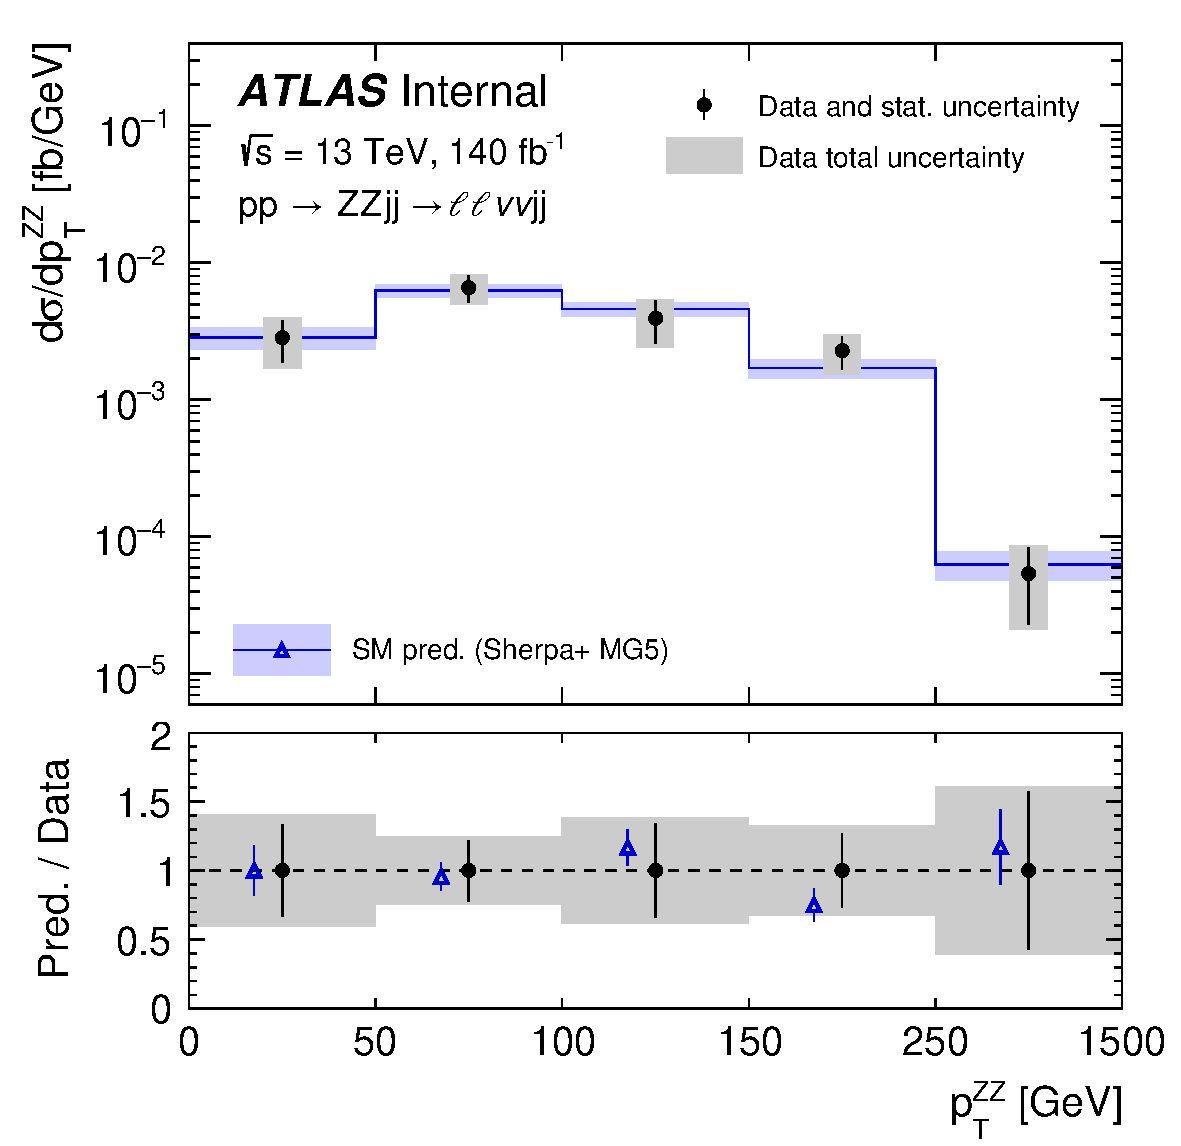
\includegraphics[width=0.35\linewidth]{figures/ch5-llvv/diff-xs/ZZjj-pT-ZZ.pdf}
    }
    \subfloat[]{      
    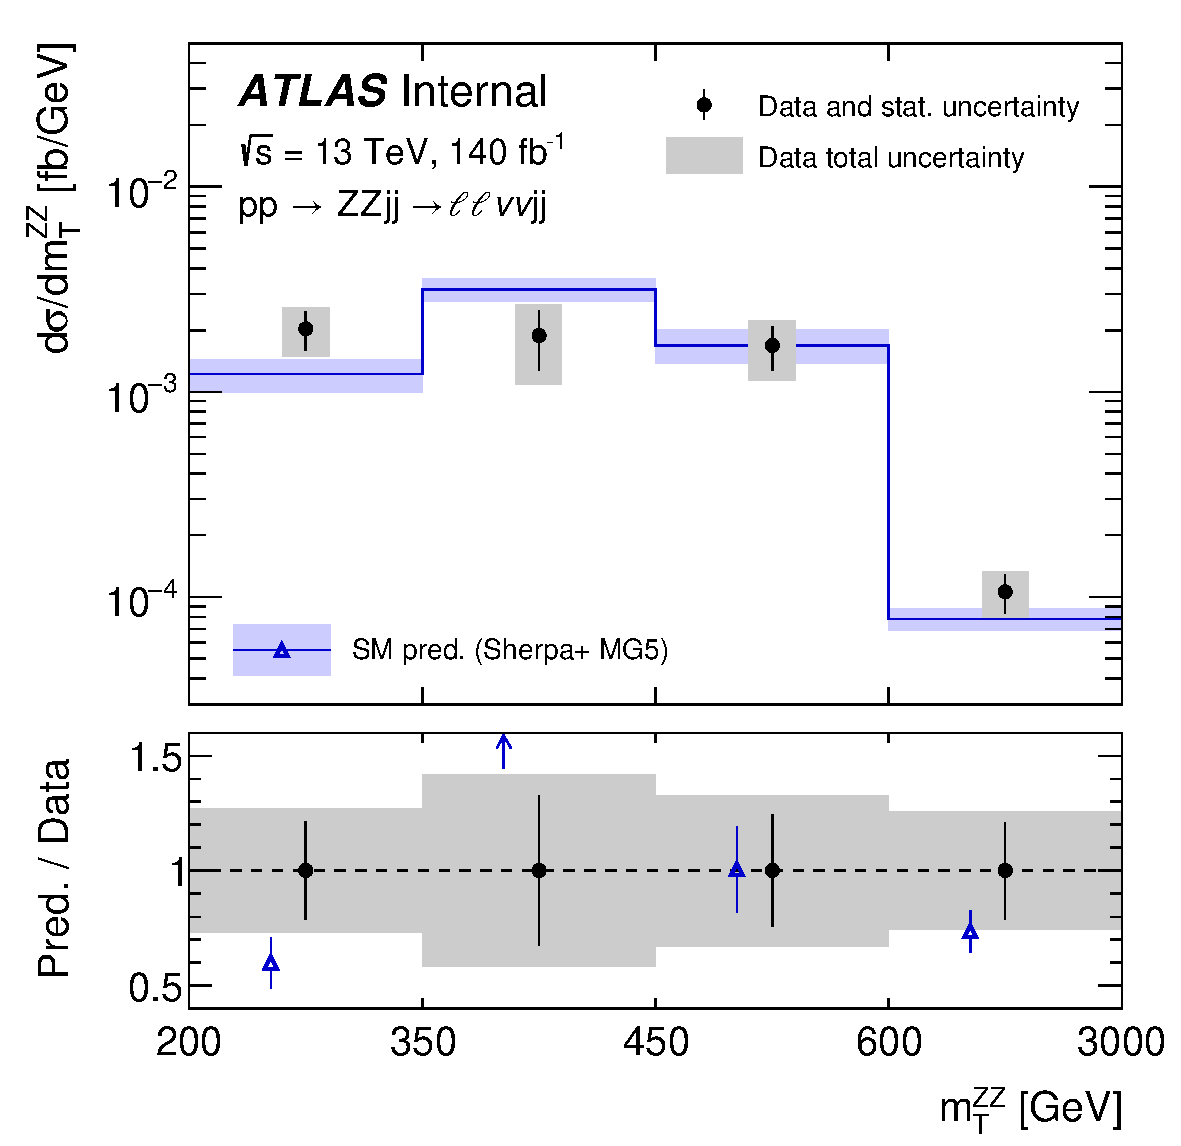
\includegraphics[width=0.35\linewidth]{figures/ch5-llvv/diff-xs/ZZjj-mT-ZZ.pdf}
    }\\
            \subfloat[]{  
    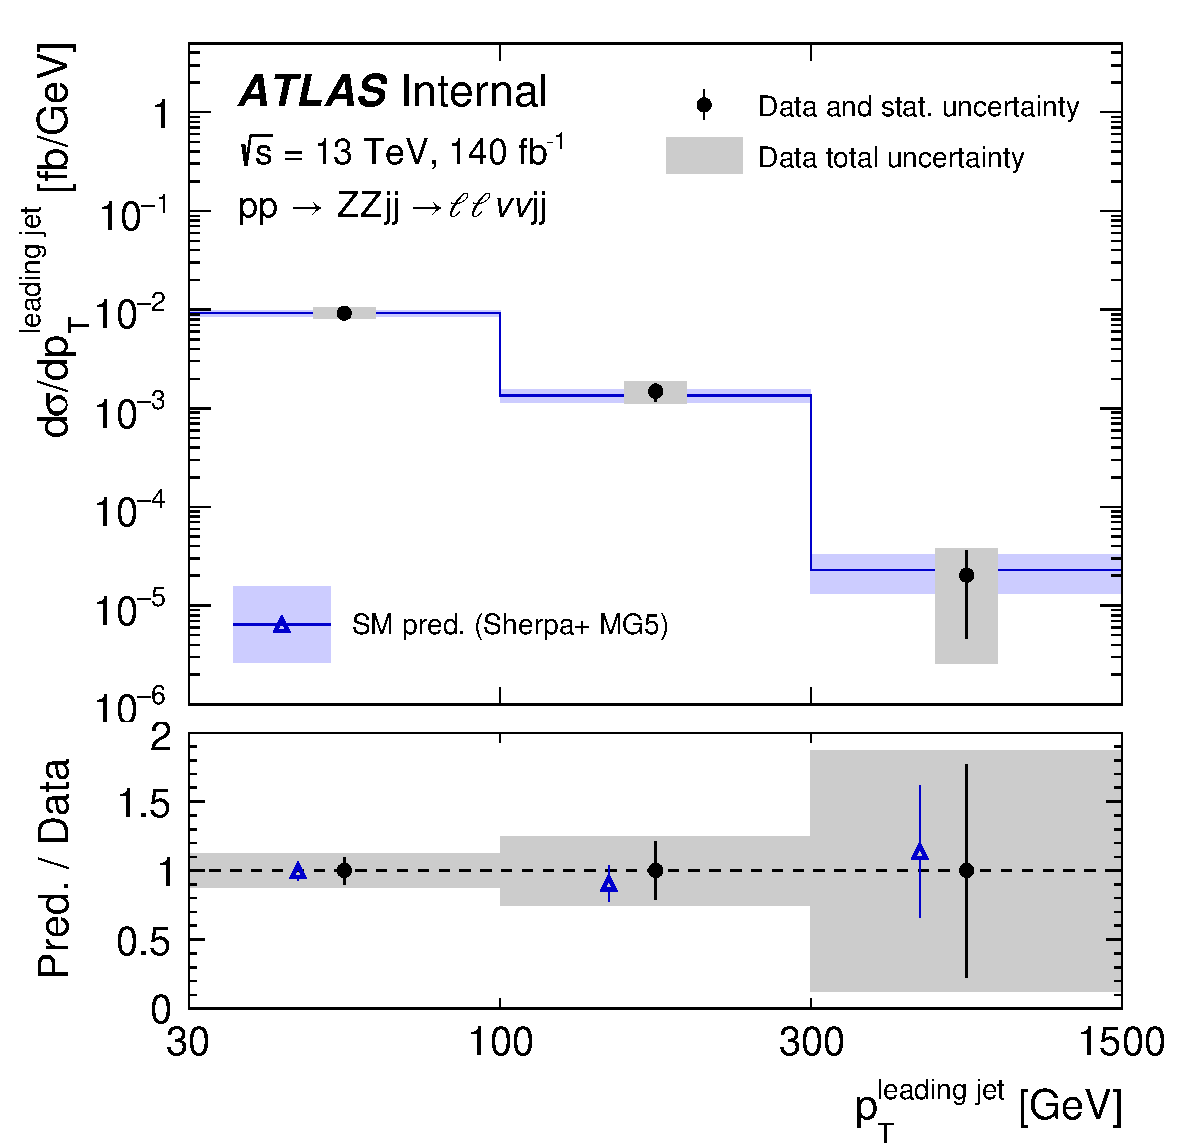
\includegraphics[width=0.35\linewidth]{figures/ch5-llvv/diff-xs/ZZjj-pT-j1.pdf}
    }
            \subfloat[]{  
    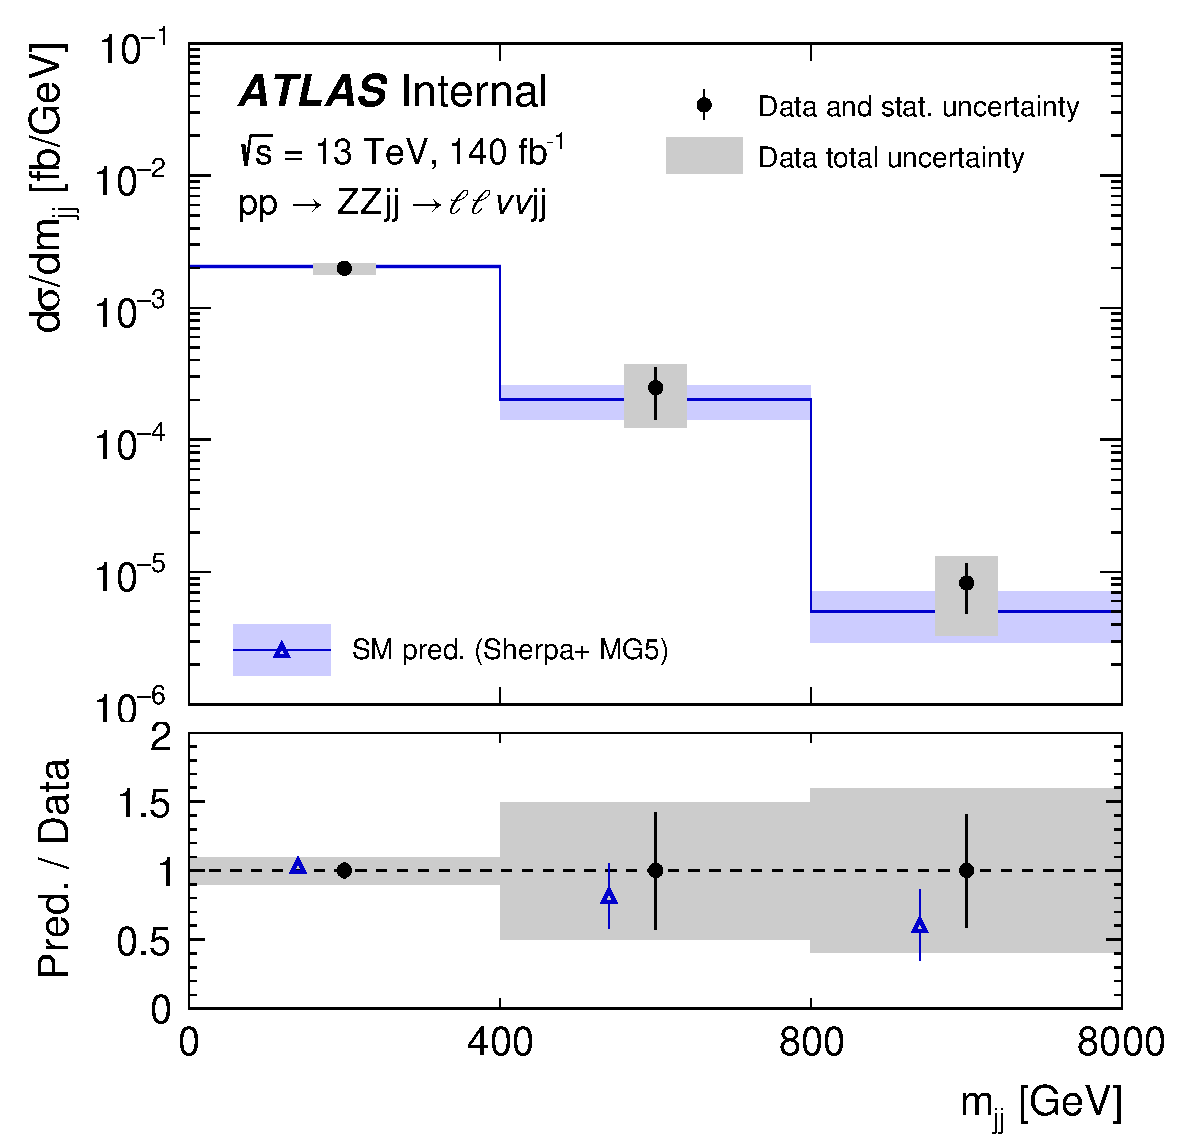
\includegraphics[width=0.35\linewidth]{figures/ch5-llvv/diff-xs/ZZjj-mjj.pdf}
    }
    \caption{Differential cross-section measurements in the $ZZjj \rightarrow \ell\ell\nu\nu jj$ fiducial phase space, compared with SM predictions for a set of kinematic variables:
     $ \text{(a)}~p_\text{T}^\text{Z},~
       \text{(b)}~\Delta\phi(\ell, \ell),~
       \text{(c)}~|y^Z|,~
       \text{(d)}~p_\text{T}^\text{ZZ},~
       \text{(e)}~m_\text{T}^\text{ZZ},~
       \text{(f)}~p_\text{T}^\text{leading-jet},~
       \text{and} ~\text{(g)}~m_\text{jj}.   
    $ 
     The SM predictions are obtained using \textsc{Sherpa} for strong production and \textsc{MadGraph5} for electroweak production. 
     The statistical and total uncertainties on the data points are displayed in both the differential cross-sections and the corresponding ratios. The total theoretical uncertainties for the  MC predictions are represented as shaded bands in the cross-section panels and as error bars in the ratio panels.
    }
\label{fig:diff-xs-ZZjj}
\end{figure}



%%%%%%%%%%%%%%%%%%%%%%%%%%%%%%%%%%%%%%%%%%%%%%%%%%
%\section{Results}
%\label{sec:llvv_results}

%This section presents the results of the inclusive $ZZ \to \ell\ell\nu\nu$ analysis performed on the full Run 2 dataset, corresponding to an integrated luminosity of $140~\text{fb}^{-1}$. The measurements include the extraction of signal strengths via a profile-likelihood fit, the determination of fiducial and total integrated cross-sections, and the measurement of differential cross-sections unfolded to particle level. Finally, limits are placed on anomalous neutral triple gauge couplings (aTGCs) within the Effective Field Theory (EFT) framework.

%\subsection{Signal Extraction and Fit Results}
%\label{subsec:signal_extraction}

%The signal yield is extracted using a binned profile-likelihood fit to the discriminative observable $\Delta\phi(\ell\ell, E_{\mathrm{T}}^{\text{miss}})$. This fit is performed simultaneously across the Signal Region (SR) and the dedicated Control Regions (CRs) described in Section~\ref{sec:llvv_event_selection}. 

%The observed signal strength parameter, defined as the ratio of the observed signal yield to the Standard Model (SM) prediction ($\mu = \sigma_{\text{obs}}/\sigma_{\text{exp}}$), is measured to be:
%\begin{equation}
%    \mu_{ZZ} = 1.05 \pm 0.05,
%\end{equation}
%indicating excellent agreement with the SM expectation. The dominant background normalization factors constrained by the fit are found to be close to unity, with $\mu_{WZ} = 1.00^{+0.06}_{-0.05}$ and $\mu_{\text{top}} = 0.98^{+0.13}_{-0.10}$. The normalization for the $Z+\text{jets}$ background varies by jet multiplicity, ranging from $1.14$ in the 0-jet region to $1.10$ in the $\geq 2$-jet region.

%The post-fit distribution of $\Delta\phi(\ell\ell, E_{\mathrm{T}}^{\text{miss}})$ in the signal region is shown in Figure~\ref{fig:postfit_observed}. The data is well-described by the post-fit predictions within the assigned uncertainties. Representative kinematic distributions, such as the transverse mass of the $ZZ$ system ($m_{\mathrm{T}}^{ZZ}$) and the transverse momentum of the leading lepton, are shown in Figure~\ref{fig:postfit_observed}.

%\begin{figure}[!htbp]
%    \centering
%    \subfloat[]{
%        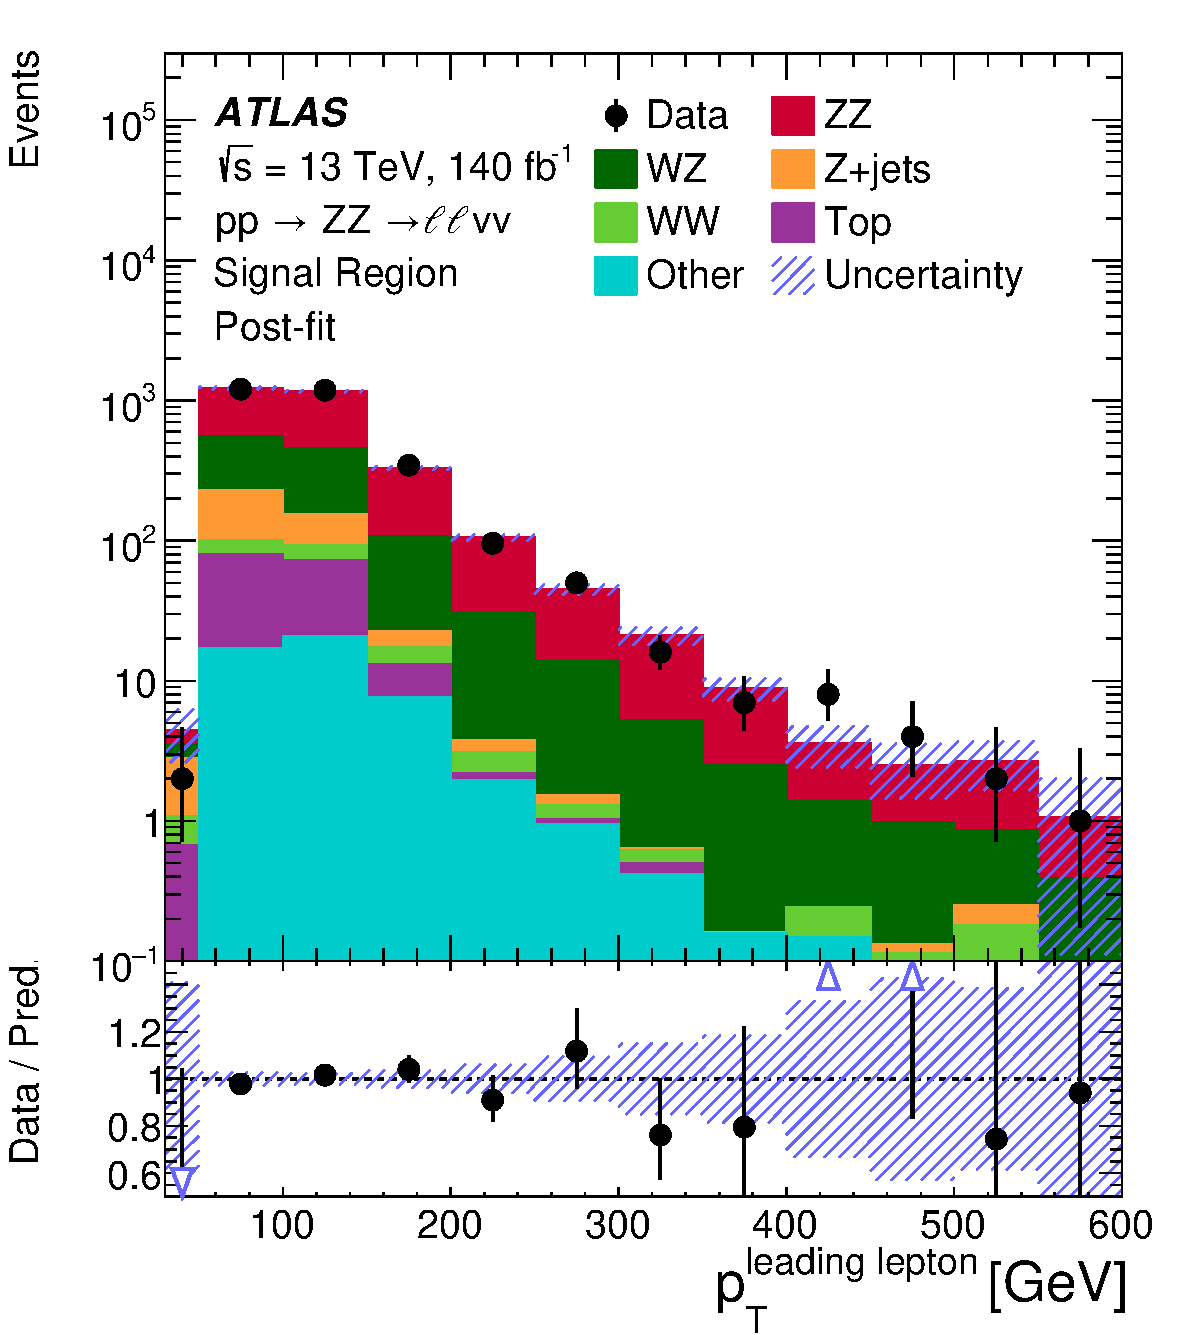
\includegraphics[width=0.3\linewidth]{figures/ch5-llvv/fig_postfit_a.pdf}
%        \label{fig:postfit_leading_lep_pt}
%    }
%    \hfill
%    \subfloat[]{
%        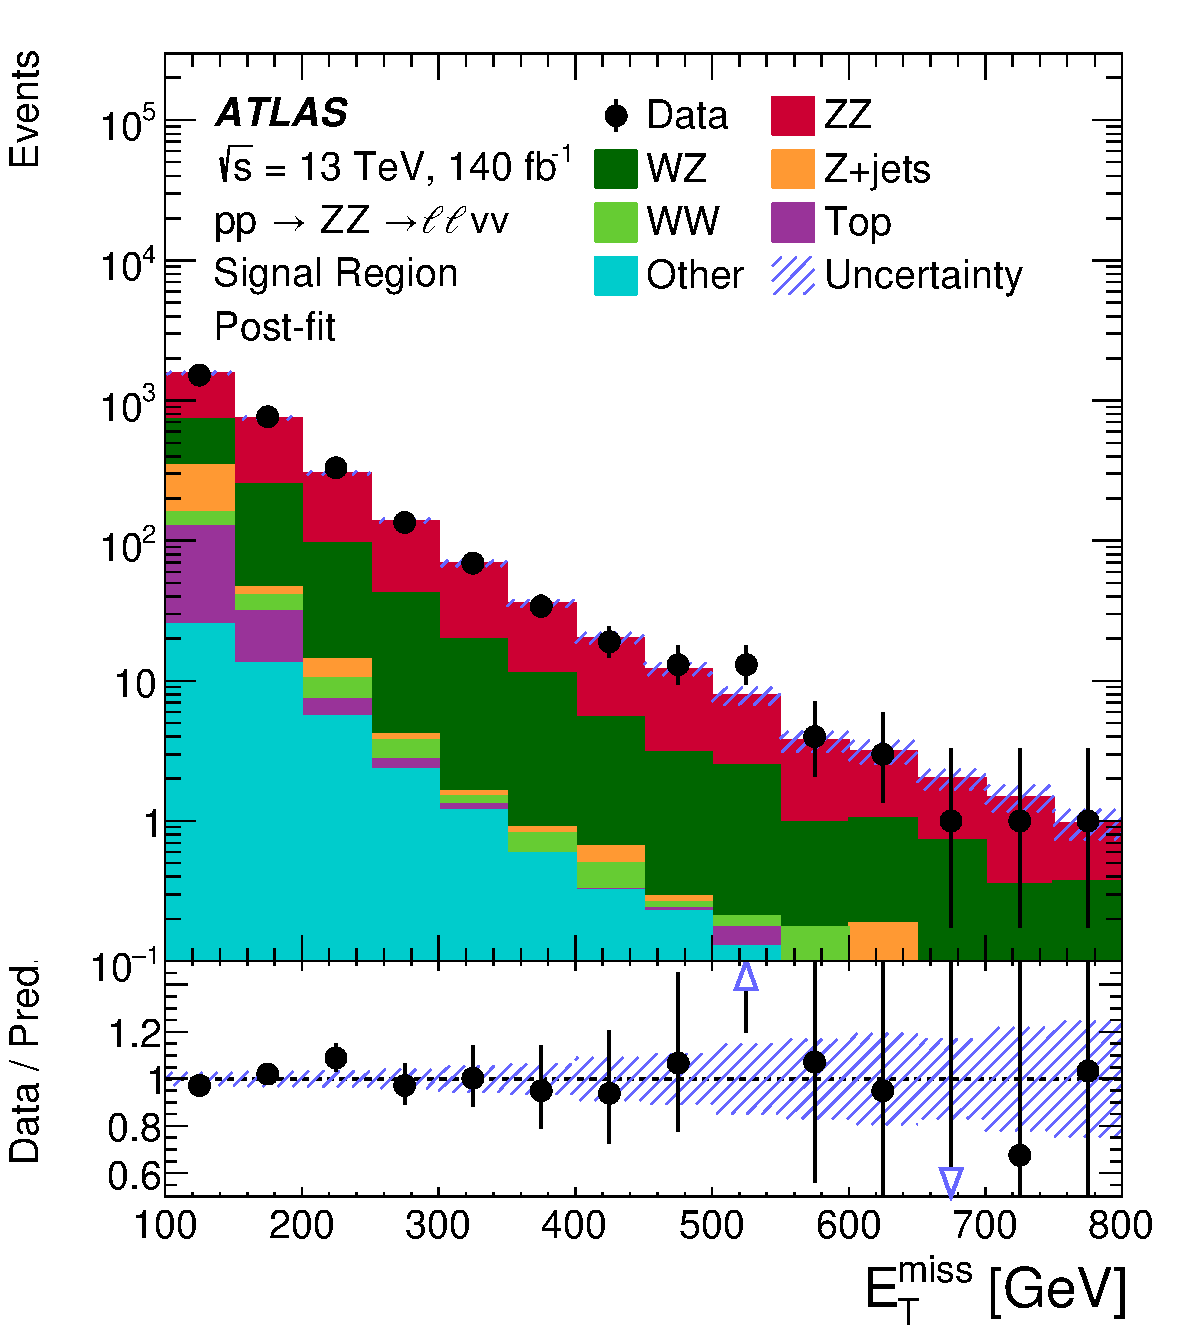
\includegraphics[width=0.3\linewidth]{figures/ch5-llvv/fig_postfit_b.pdf}
%        \label{fig:postfit_met}
%    }
%    \hfill
%    \subfloat[]{
%        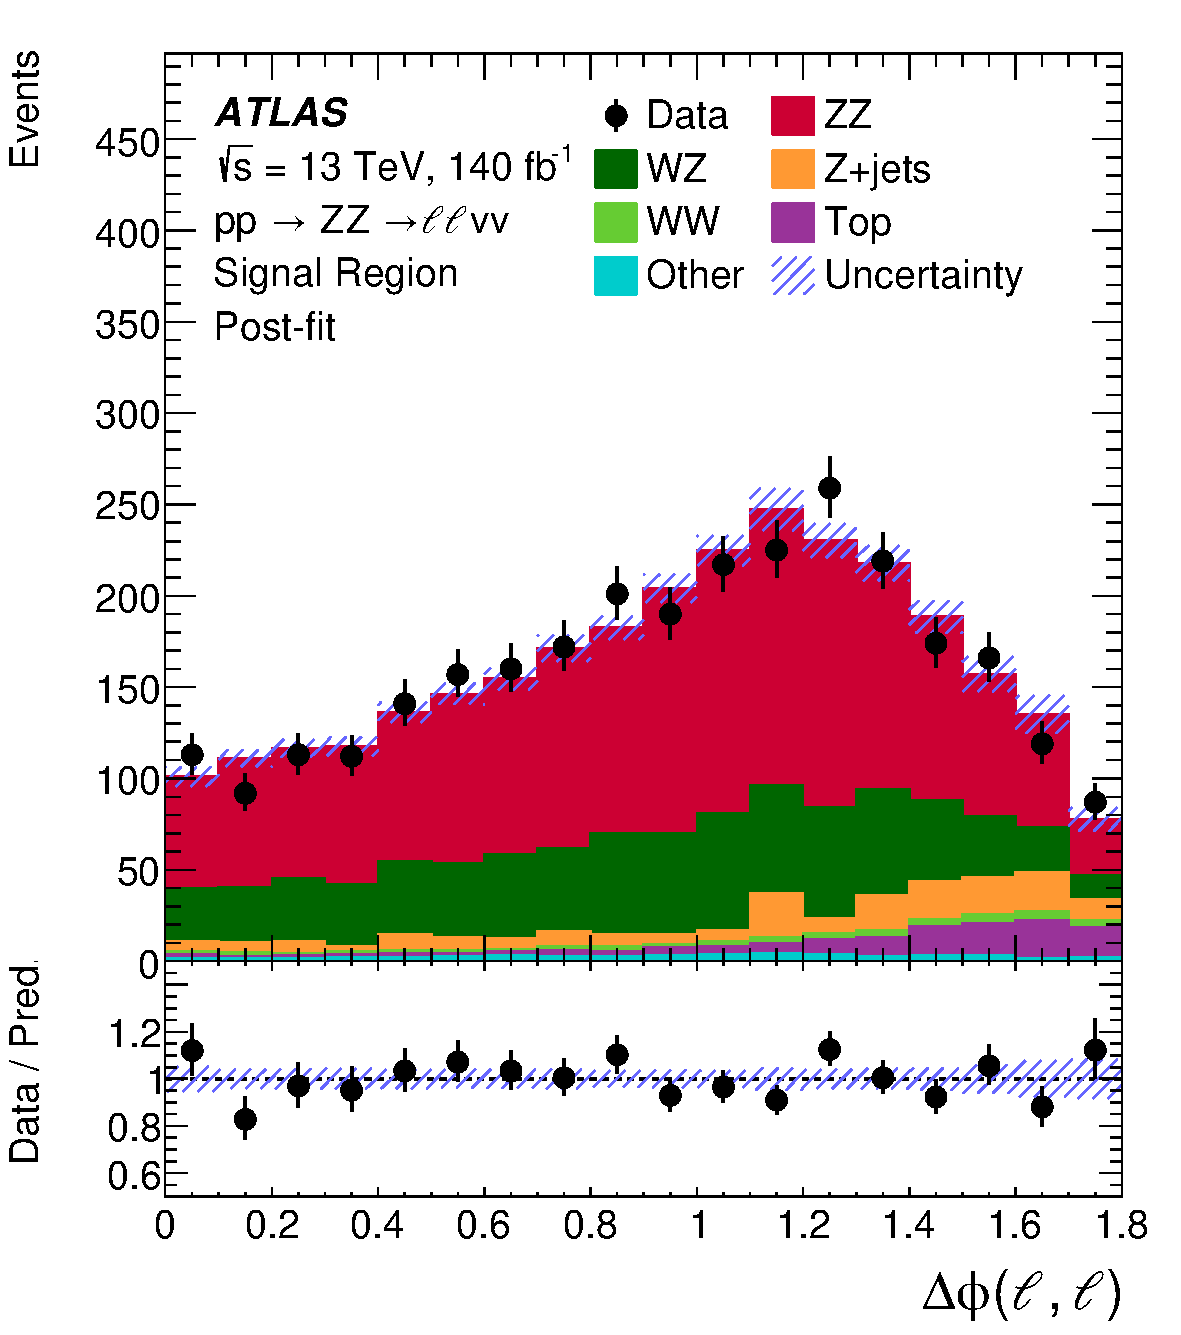
\includegraphics[width=0.3\linewidth]{figures/ch5-llvv/fig_postfit_c.pdf}
%        \label{fig:postfit_dphi_ll}
%    }    
%    \caption{Post-fit kinematic distributions for the inclusive $ZZ$ SR
%    (a) the transverse momentum of the leading lepton $p_\text{T}^\text{leading lepton}$, 
%    (b) $E_\text{T}^\text{miss}$, and 
%    (c) the azimuthal angle separation between two charged leptons $\Delta\phi(\ell, \ell)$. 
%    The data points are shown with statistical error bars, while the shaded band represents the total post-fit uncertainty in the prediction, combining statistical and systematic uncertainties. Open markers indicate data points lying outside the vertical range of the plot.}
%    \label{fig:postfit_observed}
%\end{figure}

%\subsection{Integrated Cross-Section Measurements}
%\label{subsec:integrated_xsec}

%The measured signal strength is converted into a fiducial cross-section using the SM predictions from \textsc{Sherpa} and \textsc{MadGraph5}. 

%The measured fiducial cross-section for the inclusive $ZZ \to \ell\ell\nu\nu$ process is:
%%    \sigma_{ZZ \to \ell\ell\nu\nu}^{\text{fid}} = 21.0 \pm 1.0~\text{fb}.
%\end{equation}
%The total uncertainty is composed of $\pm 0.73$ (stat), $\pm 0.57$ (exp), $\pm 0.18$ (theory), and $\pm 0.18$ (lumi) fb. This result represents a significant improvement in precision compared to previous ATLAS measurements using partial Run 2 data, with the total uncertainty reduced from 7.0\% to approximately 4.8\%. 

%The measurement is consistent with the state-of-the-art SM prediction calculated using \textsc{Matrix} at NNLO in QCD and NLO in EW corrections, which yields $21.03 \pm 0.30$ fb.

%Using the fiducial acceptance factor $A_{ZZ}$ and the branching ratio for $ZZ \to 2\ell 2\nu$, the result is extrapolated to the full phase space for $Z$ boson masses between 66 and 116 GeV. The total $pp \to ZZ$ cross-section is determined to be:
%\begin{equation}
%    \sigma_{pp \to ZZ}^{\text{total}} = 15.38 \pm 0.81~\text{pb},
%\end{equation}
%which agrees well with the \textsc{Matrix} prediction of $15.40 \pm 0.38$ pb.


\section{Constraints on Anomalous Gauge Boson Self-interaction Couplings}
\label{subsec:anom_couplings}

As presented in the sections above, the measured fiducial and total cross-sections are in good agreement with the SM predictions within the measurement uncertainties. These results enable constraints to be placed on anomalous gauge boson self-interaction couplings.

Inclusive $ZZ$ production (particularly see diagram in Figure~\ref{fig:zz-prod} (c)) provides a key channel for probing anomalous neutral triple gauge couplings (aNTGCs). In the SM, the $s$-channel diagram involving the neutral $ZZZ$ or $ZZ\gamma$ vertex is absent, making this process particularly sensitive to possible deviations from SM expectations.

The $ZZjj$ production in $pp$ collisions (see Figure~\ref{fig:zzjj-prod}) includes electroweak vector boson scattering (VBS) processes that involve the triple gauge boson ($WWZ$) and quartic gauge boson ($WWZZ$) couplings. These processes are directly linked to two fundamental aspects of the SM electroweak theory, the non-Abelian gauge structure and spontaneous electroweak symmetry breaking, and therefore provide sensitivity to both anomalous triple gauge couplings (aTGCs) and anomalous quartic gauge couplings (aQGCs).

Since no unified framework simultaneously describing aTGCs and aQGCs is currently available, the inclusive $ZZ$ measurement is used to constrain aTGCs, while the $ZZjj$ process is used to search for aQGCs.

Simulation samples for aTGC and aQGC interpretations are generated using the decomposition method, in which the matrix element is expressed as
\begin{equation}
\small
    |A_{\text{SM}} + \sum_i c_i A_i|^2
    = |A_{\text{SM}}|^2
    + \sum_i c_i\, 2\, \mathrm{Re}(A_{\text{SM}} A_i^*)
    + \sum_i c_i^2 |A_i|^2
    + \sum_{i \ne j} c_i c_j\, 2\, \mathrm{Re}(A_i A_j^*),
\end{equation}\label{eq:BSM}
where $A_{\text{SM}}$ denotes the SM amplitude, $A_i$ the beyond-the-SM (BSM) contributions, and $c_i$ the corresponding coupling coefficients. 
The first term represents the pure SM contribution. The second term corresponds to the interference between the SM and each BSM amplitude (linear term), while the third term represents the pure BSM contribution from each operator (quadratic term). The final term describes the interference between different BSM amplitudes. For both the aTGC and aQGC interpretations, all BSM contributions in Eq.~\ref{eq:BSM} are included, namely the linear interference terms ($c_i$), the quadratic terms ($c_i^2$), and the cross-interference terms ($c_i c_j$).

Limits are derived under the linear+quadratic assumption, in which both the interference between SM and BSM operators and the quadratic contributions of the BSM operators are retained in the cross-section prediction. For both the aTGC and aQGC interpretations, detector-level distributions are used as inputs to the fit, enabling optimised binning in the most sensitive regions while avoiding additional uncertainties associated with unfolding.

%%%%%%%%%%%%%%%
\subsection{Constraints on Anomalous Neutral Triple Gauge Couplings}
\label{sec:aTGC}

Inclusive $ZZ$ production is sensitive to anomalous $ZZZ$ and $ZZ\gamma$ couplings (aTGCs). Constraints are derived by fitting the reconstructed transverse momentum distribution of the dilepton system, $p_{\mathrm{T}}^{Z}$, shown in Figure~\ref{fig:ptll-aTGC}. No significant deviations from the SM prediction are observed in the high-$p_{\mathrm{T}}$ tails, where sensitivity to aTGC effects is enhanced.

\begin{figure}
    \centering
    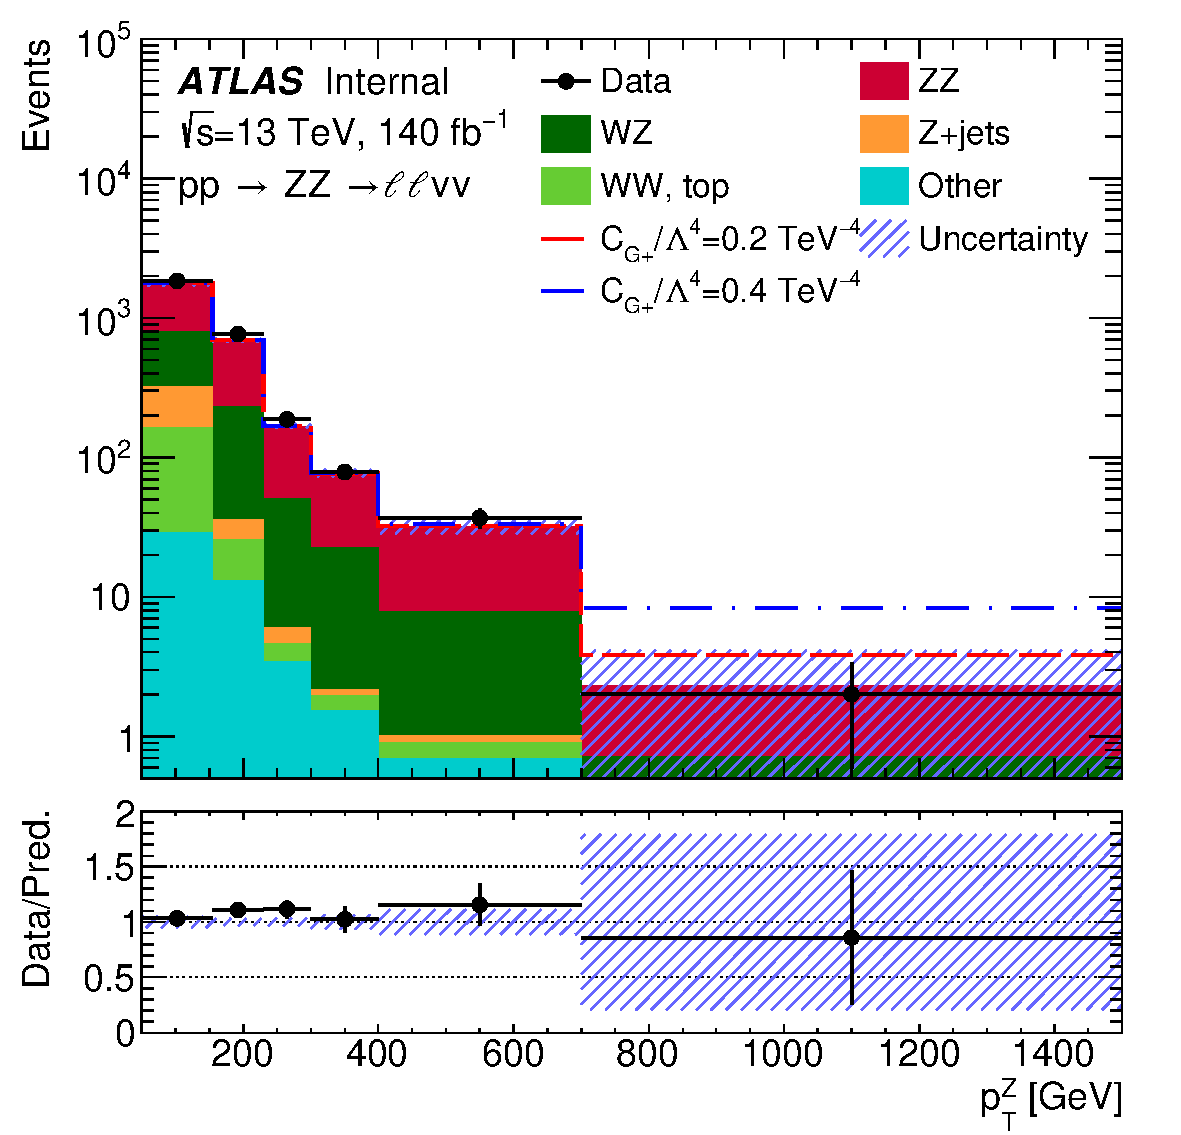
\includegraphics[width=0.6\linewidth]{figures/ch5-llvv/aTGC-aQGC/ptll_atgc.pdf}
    \caption{Distribution of the transverse momentum of the dilepton system, $p_\text{T}^{Z}$, including data and SM predictions.
    The dashed band represents the total systematic uncertainty in the SM prediction. The expected effects of an aTGC induced by the operator $O_{G+}$, for two representative values of the Wilson coefficient, are also shown.}
    \label{fig:ptll-aTGC}
\end{figure}

Limits on aTGC parameters are derived using two complementary frameworks: the vertex-function (VF) formalism~\cite{Baur2000,Biekotter2021} and the Standard Model Effective Field Theory (SMEFT)~\cite{Degrande:2013,Degrande2014,Ellis2023}. 

The most general anomalous $ZZV$ ($V=Z,\gamma$) vertex function for on-shell $Z$ bosons is given by~\cite{Hagiwara:1986vm}:
\begin{equation}
g_{ZZV}\Gamma_{ZZV}^{\alpha\beta\mu}
= e\frac{P^2-m_V^2}{m_Z^2}
\left[
if_4^V(P^{\alpha}g^{\mu\beta}+P^{\beta}g^{\mu\alpha})
+ if_5^V\epsilon^{\mu\alpha\beta\rho}(q_1-q_2)_\rho
\right],
\label{eqn:vtx_func}
\end{equation}
where $P$, $q_1$, and $q_2$ denote the momenta of the $V$ boson and the two on-shell $Z$ bosons, respectively. The anomalous couplings $f_4^V$ and $f_5^V$ correspond to CP-violating and CP-conserving interactions.

In the SMEFT framework, the Lagrangian is extended by dimension-eight operators:
\begin{equation}
\mathcal{L}_\text{SMEFT}
= \mathcal{L}_\text{SM}
+ \sum_i \frac{C_i}{\Lambda^4}\mathcal{O}_i^{(8)},
\label{eqn:eft}
\end{equation}
where $\mathcal{O}_i^{(8)}$ are dimension-eight operators and $C_i$ their Wilson coefficients. This analysis includes the operators 
$\mathcal{O}_{G+}$, $\mathcal{O}_{G-}$, $\mathcal{O}_{\widetilde{B}W}$, 
$\mathcal{O}_{BB}$, $\mathcal{O}_{BW}$, and $\mathcal{O}_{WW}$ with corresponding coefficients $C_i/\Lambda^4$~\cite{Degrande2014,Ellis2023}. 
The new-physics scale is fixed to $\Lambda = 1$~TeV.

The 95\% confidence level (CL) intervals for the VF parameters $f_4^{\gamma/Z}$ (CP-violating) and $f_5^{\gamma/Z}$ (CP-conserving), as well as for the SMEFT higher-dimensional operator coefficients, are presented in Table~\ref{tab:atgc_limits}. The results from the VF framework improve upon the previous ATLAS $ZZ \to \ell\ell\nu\nu$ measurement by approximately a factor of 1.7. The limits of the SMEFT coefficients are derived for the first time in this channel.

\begin{table}[htbp]
\centering
\scriptsize
\renewcommand{\arraystretch}{1.5}
\begin{tabular}{lccc}
\hline
\textbf{Model} & \textbf{Coefficient} & \textbf{Expected} & \textbf{Observed} \\
\hline
VF & $f_{4}^{\gamma}$ & $[-7.7,\ 7.7] \times 10^{-4}$ & $[-6.4,\ 6.4] \times 10^{-4}$ \\
VF & $f_{4}^{Z}$      & $[-6.8,\ 6.8] \times 10^{-4}$ & $[-5.7,\ 5.7] \times 10^{-4}$ \\
VF & $f_{5}^{\gamma}$ & $[-7.8,\ 7.7] \times 10^{-4}$ & $[-6.4,\ 6.5] \times 10^{-4}$ \\
VF & $f_{5}^{Z}$      & $[-6.9,\ 6.9] \times 10^{-4}$ & $[-5.8,\ 5.8] \times 10^{-4}$ \\
\hline
SMEFT &  $C_{G+}/\Lambda^4$         & $[-0.36,\ 0.36]$ & $[-0.29,\ 0.30]$ \\
SMEFT &  $C_{G-}/\Lambda^4$         & $[-1.1,\ 1.2]$   & $[-0.95,\ 0.95]$ \\
SMEFT & $C_{\tilde{B}W}/\Lambda^4$ & $[-1.3,\ 1.3]$   & $[-1.1,\ 1.1]$ \\
SMEFT &  $C_{BB}/\Lambda^4$         & $[-1.6,\ 1.6]$   & $[-1.3,\ 1.3]$ \\
SMEFT &  $C_{BW}/\Lambda^4$         & $[-2.9,\ 2.9]$   & $[-2.4,\ 2.4]$ \\
SMEFT & $C_{WW}/\Lambda^4$         & $[-2.4,\ 2.4]$   & $[-2.0,\ 2.0]$ \\
\hline
\end{tabular}
\caption{\rm Expected and observed 95\% CL intervals for the parameters of the VF and SMEFT formalisms derived from inclusive $ZZ$ production, obtained without applying any unitarization procedure. The limits are derived by varying one parameter at a time while setting all other aTGC parameters to zero.}
\label{tab:atgc_limits}
\end{table}






